\subsection{GANs}\label{sec:gans}
Generative adversarial networks (GANs), first proposed by \cite{goodfellow2014generative}, have revolutionized the field of generative modeling in deep learning. A GAN consists of two adversarial models, a \textit{Generator} $G$ and a \textit{Discriminator} $D$. The generator aims to capture the data distribution and thus be able to produce data that mimics the real data. It takes data sampled from a prior distribution $\mathcal{Z}$, often a Gaussian distribution, and learns a function to map it into the data space. The discriminator model $D$ simultaneously aims to distinguish between data from the real distribution and data generated by $G$. To enable $G$ to learn the real data distribution and $D$ to improve its discriminative power, a non-cooperative two-player minimax game is used in combination with simultaneous gradient descent \citep[p.5]{saxena2021generative}. The objective function of a basic GAN model uses two objectives: Parameters of $D$ ($\theta_D$) are chosen such that the negative log-likelihood for binary classification is minimized and parameters of $G$ ($\theta_G$) are chosen such that the generated examples have a high probability of being real \citep[p.6]{saxena2021generative}. Thus, the overall objective function can be formulated as
\begin{equation}
\label{eq:basic_gan_loss}
\min_{\theta_G} \max_{\theta_D} V(G, D) = \min_G \max_D \mathbb{E}_{x \sim p_{\text{data}}} [\log D(x)] + \mathbb{E}_{z \sim p_z} [\log (1 - D(G(z)))]
\end{equation}
 where $V(G,D)$ is a binary cross entropy function \citep[p.6]{saxena2021generative}. In the beginning, none of the networks has any knowledge about the domain \citep[p.2]{bermano2022state}. The models improve by learning from each other. \cite{bermano2022state} describe the training as a repetitive process, in which the generator tries to fool the discriminator which in turn learns to recognize this strategy. This training scheme allows the model to learn via self-supervision and interestingly, the generator learns to generate high-fidelity images without ever seeing a single real image \citep[p.2]{bermano2022state}. As an extension, \cite{mirza2014conditional} introduced a conditional GAN architecture, where a conditioning of a single class of the domain can be achieved in both the generator and discriminator. Since in this work I focus on across-class manipulations, unconditional architectures are used which can capture the multimodal distribution of multiple classes in one model. The basic GAN architecture can be seen in figure \ref{fig:gan_architecture}.
 
\begin{figure}[ht]
    \centering
    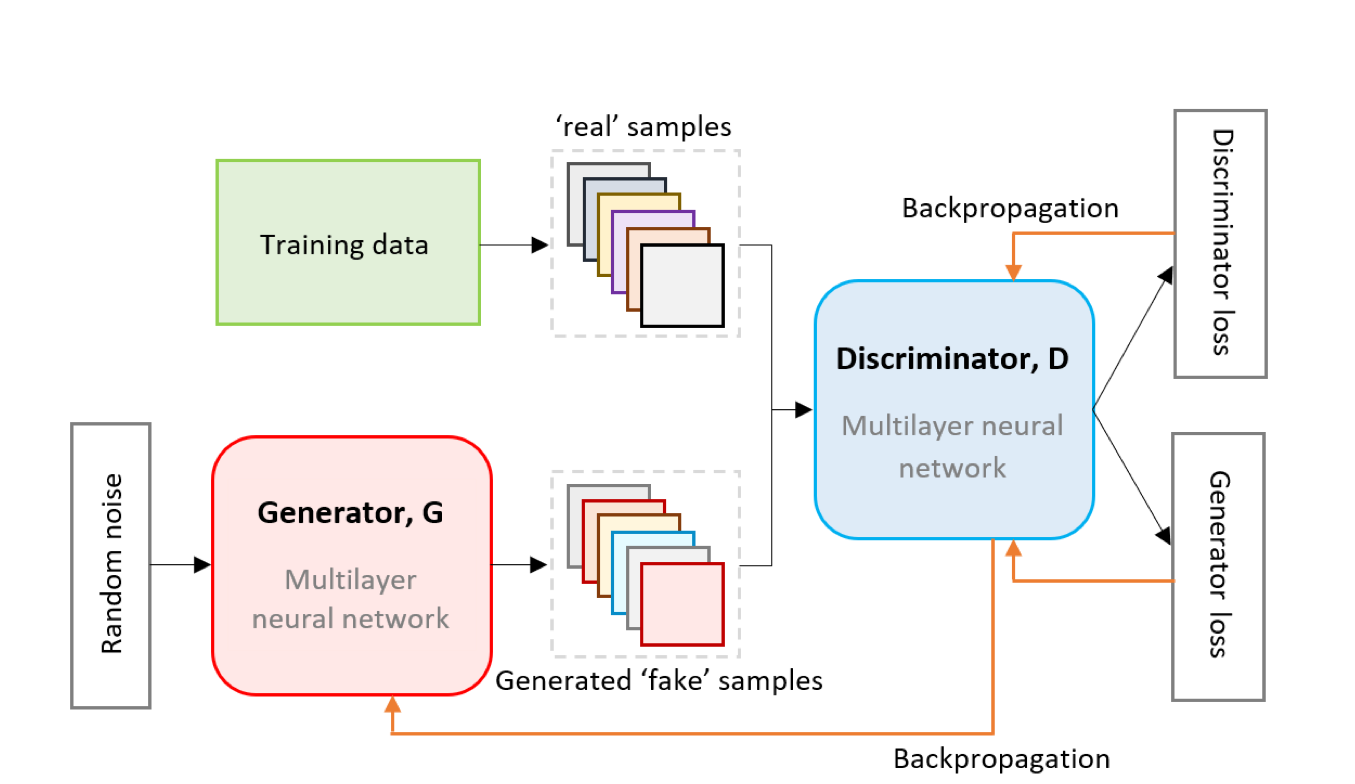
\includegraphics[width=0.8\linewidth]{Thesis/Background/assets/basic_gan_architecture.png}
    \caption[Basic GAN architecture]{Basic GAN architecture - taken from \cite{little2021generative}} 
    \label{fig:gan_architecture}
\end{figure}
% While all GAN architectures share the concept of two adversarial networks, there are many combinations of generator architectures, discriminator architectures, loss functions, and optimization algorithms. Most image generation architectures use deep neural networks for both the generator and discriminator. Given the vastness of GAN architectures, I will focus on the key improvements relevant to the architecture used in this work. DCGAN, proposed by \cite{radford2015unsupervised}, uses deep convolutional networks in the generator and discriminator, forming the foundation for many subsequent high-fidelity image generation GANs. \cite{arjovsky2017wasserstein} and \cite{gulrajani2017improved} introduced improvements in discriminator loss formulation and optimization. Since the standard GAN loss can lead to vanishing gradients with a strong discriminator \citep[p.2]{gulrajani2017improved}, they proposed using the Earth-Mover (Wasserstein) distance, resulting in the Wasserstein-GAN (WGAN), which is also used in StyleGAN. Another frequently used GAN family is based on ProGAN or progressive GAN (PGGAN), which employs a progressive growing strategy to incrementally improve the resolution of both the generator and discriminator, learning increasingly finer features \citep{karras2017progressive}. Many design choices from PGGAN, such as progressive growing, laid the foundation for StyleGAN's success.
While all GAN architectures share the concept of two adversarial networks, there are many combinations of generator architectures, discriminator architectures, loss functions, and optimization algorithms. Numerous architectures have gradually improved the image quality and training stability of GANs (e.g. DCGAN \citep{radford2015unsupervised}, WGAN \citep{arjovsky2017wasserstein}, PGGAN \citep{karras2017progressive}). The final breakthrough of image generation using GANs, however, happened with the introduction of StyleGAN \citep{stylegan1}. \\
The \textbf{StyleGAN family} (e.g., \cite{stylegan1}, \cite{stylegan2}, \cite{stylegan2ada}) has achieved an unprecedented level of image quality and fidelity \citep[p.1]{tov2021designing}. StyleGAN has become the state-of-the-art GAN architecture, and the golden standard for facial image editing \cite[p.1]{bermano2022state}. Its dominance is due to design choices that create a well-organized, smooth, and highly disentangled latent space that exhibits a semantic understanding of the target domain merely through the effect of inductive bias \citep[p.6]{bermano2022state}. A key innovation in StyleGAN is the mapping network $f: \mathcal{Z} \rightarrow \mathcal{W}$, which transforms Gaussian-distributed latent codes from $\mathcal{Z}$ into an intermediate latent space $\mathcal{W}$, ensuring better alignment with the real data distribution. This mapping allows the model to account for the non-uniform distribution of image attributes by "unwrapping" the latent space, making it more linear and easier to manage \citep[p.6]{stylegan1}. As a result, the generator can more effectively disentangle and recreate various image features, enhancing the quality and diversity of the generated images. The main component in StyleGAN's architecture is the style modulation layers that allow precise control of the "style" in generated images. The latent codes in $w$ are transformed to "styles" $\bm{y} = (y_s, y_b)$ using learned affine transformations. Using these transformations, different dimensions of the StyleGAN latent space $\mathcal{W}$ are injected at different levels of the synthesis process, allowing targeted variation at the coarse, medium, and fine details of the generated image \citep[p.4]{stylegan1}. 
\begin{wrapfigure}{r}{7cm}
    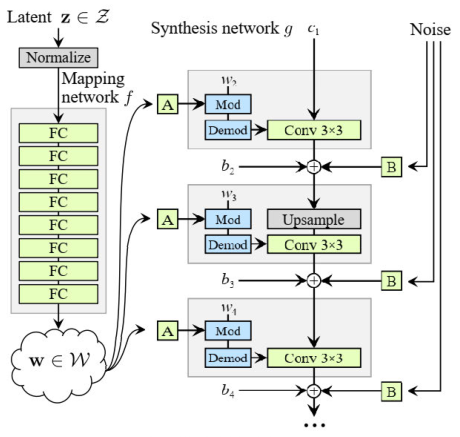
\includegraphics[width=1\linewidth]{Thesis/Background/assets/sg2_schema-cropped.pdf}
    \caption[StyleGAN2 Architecture]{StyleGAN2 Architecture - taken from \cite{hermosilla2021thermal}}
    \label{fig:stylegan2_schema}
\end{wrapfigure} 
Additionally, by injecting random noise into each layer of the synthesis network, stochastic variation in the output is ensured \citep[p.1]{stylegan2}. \\
\textbf{StyleGAN2}, an improved version of the original StyleGAN, introduces enhancements that address artifacts and improve image quality by refining both the architecture and training processes \citep[p.2]{stylegan2}. 
A key change is the replacement of progressive growing with skip-connections in the generator and a residual discriminator \citep[p.6]{stylegan2}. 
This simplifies training by maintaining a fixed resolution throughout, eliminating the need for manual tuning as resolution increases. Another major improvement is the redesign of the style modulation layers through a modulation-demodulation operation. Here, style modulation is directly applied to the convolutional layer weights, followed by demodulation to normalize feature maps. 
This enhances the consistency and quality of the generated images. A detailed schema of the StyleGAN2 architecture is shown in figure \ref{fig:stylegan2_schema}. StyleGAN2 also introduces lazy regularization, computing regularization losses every 16 minibatches, which reduces computational cost and training time \citep[p.5]{stylegan2}. 
Additionally, the novel path length regularization ensures that small changes in the latent code $w \in \mathcal{W}$ lead to smooth, small changes in the generated image. This regularizer penalizes large variations in the perceptual space of consecutive latent codes during training, resulting in more reliable models and smoother generators, which are easier to invert \citep[p.5]{stylegan2}. Since the model in this work needs to produce subtle changes when manipulating images, smooth latent space interpolation, achieved by StyleGAN2's path length regularizer, is crucial.

\textbf{StyleGAN2Ada} \citep{stylegan2ada} is a modified version of StyleGAN2 which introduces adaptive data augmentation techniques to address overfitting and improve generalization. Training GANs with a small dataset can easily lead to discriminator overfitting and thus training of the generator fails due to vanishing gradients. Using adaptive discriminator augmentations, the authors can stabilize training on small datasets and show that only a few thousand images are needed to train StyleGAN2Ada \citep[p.1]{stylegan2ada}. This is achieved through the use of an adaptive augmentation pipeline that introduces random transformations, such as translation, rotation, and color jittering, only when the discriminator begins to overfit. Since in this work, a limiting factor is the access to high-quality training data, using StyleGAN2Ada is the logical choice, as it allows training of a high-quality generator on a small sample. 






